%%%%%%%%%%%%%%%%%%%%%%%%%%%%%%%%%%%%%%%%%%%%%%%%%%%%%%%%%%%%%%%%%
\section{Load time performance on top websites} \label{performance}
%%%%%%%%%%%%%%%%%%%%%%%%%%%%%%%%%%%%%%%%%%%%%%%%%%%%%%%%%%%%%%%%%

\sys's performance goal is to provide its security guarantees without
impacting the user's browsing experience. We now briefly report \sys's
impact on top website load times, representing the expected behaviour
of a user's average web browsing experience. For more performance
evaluation results please see ~\autoref{appendix:perf-eval}.

%  \label{top_sites}
%% We first report our extension's impact on top website load times,
%% representing the expected behaviour of an user's average web browsing
%% experience. 
% 
For these tests we used the top 500 websites as
reported by Moz.com~\cite{top500}. For each website, we loaded it 25
times (with a 25 second timeout) and recorded the following values:
requestStart, responseEnd, domComplete, and decodedBodySize. From the
initial set of 500, we only report values for 441: the other 59 had
consistent issues with timeouts, insecure certificates, and network
errors. In our setup, we used a headless version of Firefox 69.0, and
Selenium WebDriver for NodeJS, with GeckoDriver. All experiments were
run on one machine with an Intel Xeon CPU E5-2407 2.40GHz processor,
32 GB DRAM, and our university's 1GiB connection.

We ran four test suites:
\textbf{No extension cold cache}: Firefox is loaded without the extension installed and the web driver is re-instantiated for every page load.
\textbf{Extension cold cache}: As before, but Firefox is loaded with the extension installed.
\textbf{No extension warm cache}: Firefox is loaded without the extension installed and the same web driver is used for the page's 25 loads.
\textbf{Extension warm cache}: As before, but Firefox is launched with the extension installed.

For each set of tests, we reduced the recorded values to two comparisons: network filter (responseEnd - requestStart), and page ready (domComplete - responseStart). The first analyzes the time spent by the network filter, while the second determines the time spent until the whole document has loaded. We calculate the medians for each website for each of these measures as well as the decodedByteSize.

\begin{figure}[h]
		\begin{center}
	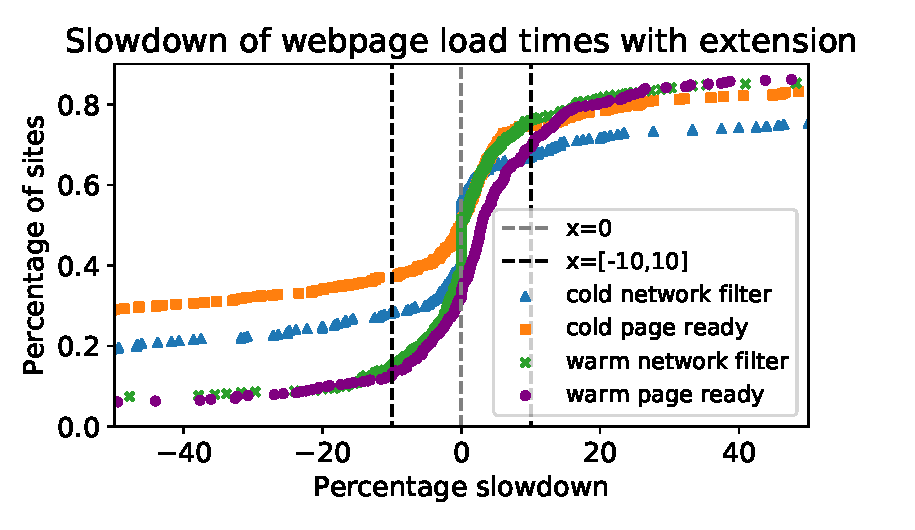
\includegraphics[scale=0.5]{results/extension_slowdown_overall_small.pdf}
	\caption{Cumulative distribution of relative percentage slowdown with extension installed for top sites.}
	\label{fig:overall_slowdown}
\end{center}
	
\end{figure}

We compare the load times with/without the extension by calculating the relative slowdown with the extension installed according to the following formula:

\begin{equation*}
100*\frac{\tilde{x}_{with}-\tilde{x}_{without}}{\tilde{x}_{without}}
\end{equation*}
\\
where $\tilde{x}$ is the median with/without the extension running.

\autoref{fig:overall_slowdown} plots the results. The graph
shows a slowdown of less than 10\% for 72.6\% of sites, and less than
50\% for 82\% of sites when the extension is running. Note that these
values are recorded as percentages, and while some are as high as
50\%, the absolute values are in 77\% of cases less than a
second. This overhead should not alter the user's experience
significantly.

The slowdown increases by at most 5\% when we take caching into
account. This is likely because the network filter causes the browser
to use less caching, especially for the DOM component, as it might
have to process it from scratch every time. While it may seem
counter-intuitive that some pages have shorter loading times with
the extension, there are several variables at play that can affect
these measurements (local network, server-side load, internal
scheduling, etc). We manually checked the websites for which values
were higher than |40\%| and verified that our extension did not change
the page's contents, a possible cause of faster load times. We also
checked the timings for the page as reported by the browser and noted
a high variance even within small time windows. The time spent by our
verification function was less than 10ms for 87.6\% of sites
(\autoref{fig:verification_time_string_length}). This corroborates our
findings that the slowdown is mostly negligible.
